%%%%%%%%%%%%%%%%%%%%%%%%%%%%%%%%%%%%%%%%%
% Proceedings of the National Academy of Sciences (PNAS)
% LaTeX Template
% Version 1.0 (19/5/13)
%
% This template has been downloaded from:
% http://www.LaTeXTemplates.com
%
% Original author:
% The PNAStwo class was created and is owned by PNAS:
% http://www.pnas.org/site/authors/LaTex.xhtml
% This template has been modified from the blank PNAS template to include
% examples of how to insert content and drastically change commenting. The
% structural integrity is maintained as in the original blank template.
%
% Original header:
%% PNAStmpl.tex
%% Template file to use for PNAS articles prepared in LaTeX
%% Version: Apr 14, 2008
%
%%%%%%%%%%%%%%%%%%%%%%%%%%%%%%%%%%%%%%%%%
%----------------------------------------------------------------------------------------
%	PACKAGES AND OTHER DOCUMENT CONFIGURATIONS
%----------------------------------------------------------------------------------------

%------------------------------------------------
% BASIC CLASS FILE
%------------------------------------------------

%% PNAStwo for two column articles is called by default.
%% Uncomment PNASone for single column articles. One column class
%% and style files are available upon request from pnas@nas.edu.

%\documentclass{pnasone}
\documentclass{pnastwo}

%------------------------------------------------
% POSITION OF TEXT
%------------------------------------------------

%% Changing position of text on physical page:
%% Since not all printers position
%% the printed page in the same place on the physical page,
%% you can change the position yourself here, if you need to:

% \advance\voffset -.5in % Minus dimension will raise the printed page on the 
                         %  physical page; positive dimension will lower it.

%% You may set the dimension to the size that you need.

%------------------------------------------------
% GRAPHICS STYLE FILE
%------------------------------------------------

%% Requires graphics style file (graphicx.sty), used for inserting
%% .eps/image files into LaTeX articles.
%% Note that inclusion of .eps files is for your reference only;
%% when submitting to PNAS please submit figures separately.

%% Type into the square brackets the name of the driver program 
%% that you are using. If you don't know, try dvips, which is the
%% most common PC driver, or textures for the Mac. These are the options:

% [dvips], [xdvi], [dvipdf], [dvipdfm], [dvipdfmx], [pdftex], [dvipsone],
% [dviwindo], [emtex], [dviwin], [pctexps], [pctexwin], [pctexhp], [pctex32],
% [truetex], [tcidvi], [vtex], [oztex], [textures], [xetex]


%------------------------------------------------
% OPTIONAL POSTSCRIPT FONT FILES
%------------------------------------------------

%% PostScript font files: You may need to edit the PNASoneF.sty
%% or PNAStwoF.sty file to make the font names match those on your system. 
%% Alternatively, you can leave the font style file commands commented out
%% and typeset your article using the default Computer Modern 
%% fonts (recommended). If accepted, your article will be typeset
%% at PNAS using PostScript fonts.

% Choose PNASoneF for one column; PNAStwoF for two column:
%\usepackage{PNASoneF}
%\usepackage{PNAStwoF}

%------------------------------------------------
% ADDITIONAL OPTIONAL STYLE FILES
%------------------------------------------------

%% The AMS math files are commonly used to gain access to useful features
%% like extended math fonts and math commands.
\usepackage{multirow}
%\usepackage{caption}
%\usepackage{subcaption}
%\usepackage{etex}
\usepackage{color}
%\usepackage[usenames,dvipsnames,svgnames,table]{xcolor}
\usepackage[usenames,dvipsnames]{xcolor}
\usepackage{tikz}
\usetikzlibrary{decorations.shapes}
\usepackage{amssymb,amsfonts,amsmath}
\usepackage{xspace}
\newcommand{\dictionary}{\ensuremath{\mathcal{D}}\xspace}


%------------------------------------------------
% OPTIONAL MACRO FILES
%------------------------------------------------

%% Insert self-defined macros here.
%% \newcommand definitions are recommended; \def definitions are supported

%\newcommand{\mfrac}[2]{\frac{\displaystyle #1}{\displaystyle #2}}
%\def\s{\sigma}

%------------------------------------------------
% DO NOT EDIT THIS SECTION
%------------------------------------------------

%% For PNAS Only:
\contributor{Submitted to Proceedings of the National Academy of Sciences of the United States of America}
\url{www.pnas.org/cgi/doi/10.1073/pnas.0709640104}
\copyrightyear{2008}
\issuedate{Issue Date}
\volume{Volume}
\issuenumber{Issue Number}

%----------------------------------------------------------------------------------------

\begin{document}

%----------------------------------------------------------------------------------------
%	TITLE AND AUTHORS
%----------------------------------------------------------------------------------------

\title{Hyperbolically speaking} % For titles, only capitalize the first letter

%------------------------------------------------

%% Enter authors via the \author command.  
%% Use \affil to define affiliations.
%% (Leave no spaces between author name and \affil command)

%% Note that the \thanks{} command has been disabled in favor of
%% a generic, reserved space for PNAS publication footnotes.

%% \author{<author name>
%% \affil{<number>}{<Institution>}} One number for each institution.
%% The same number should be used for authors that
%% are affiliated with the same institution, after the first time
%% only the number is needed, ie, \affil{number}{text}, \affil{number}{}
%% Then, before last author ...
%% \and
%% \author{<author name>
%% \affil{<number>}{}}

%% For example, assuming Garcia and Sonnery are both affiliated with
%% Universidad de Murcia:
%% \author{Roberta Graff\affil{1}{University of Cambridge, Cambridge,
%% United Kingdom},
%% Javier de Ruiz Garcia\affil{2}{Universidad de Murcia, Bioquimica y Biologia
%% Molecular, Murcia, Spain}, \and Franklin Sonnery\affil{2}{}}

\author{Justine T. Kao\affil{1}{Stanford University},
Jean Wu,\affil{1}{}
Leon Bergen\affil{2}{MIT}
\and
Noah D. Goodman\affil{1}{}}

\contributor{Submitted to Proceedings of the National Academy of Sciences
of the United States of America}

%----------------------------------------------------------------------------------------

\maketitle % The \maketitle command is necessary to build the title page

\begin{article}

%----------------------------------------------------------------------------------------
%	ABSTRACT, KEYWORDS AND ABBREVIATIONS
%----------------------------------------------------------------------------------------

\begin{abstract}
One of the biggest challenges in language understanding is that language is not always meant to be interpreted literally. In everyday situations, people often use imprecise, exaggerated, or otherwise literally false descriptions to communicate their experiences and opinions. In this paper we focus on the non-literal interpretation of number words, in particular the effects of
pragmatic halo (the imprecise interpretation of round numbers) and hyperbole (the affective subtext conveyed by exaggerated and unlikely numbers). Building on recent models of pragmatics as rational inference between speaker and listener, we model number interpretation as social inference regarding the communicative goal, meaning, and affective subtext of an utterance. Our model accurately predicts humans' pragmatic interpretation of number words, and is one of the first computational models to quantitatively capture a range of effects in non-literal language understanding.
\end{abstract}

%------------------------------------------------

\keywords{Pragmatics | Language understanding | Computational modeling} % When adding keywords, separate each term with a straight line: |

%------------------------------------------------

%% Optional for entering abbreviations, separate the abbreviation from
%% its definition with a comma, separate each pair with a semicolon:
%% for example:
%% \abbreviations{SAM, self-assembled monolayer; OTS,
%% octadecyltrichlorosilane}

% \abbreviations{}
\abbreviations{IR, Incongruity Resolution}

%----------------------------------------------------------------------------------------
%	PUBLICATION CONTENT
%----------------------------------------------------------------------------------------

%% The first letter of the article should be drop cap: \dropcap{} e.g.,
%\dropcap{I}n this article we study the evolution of ''almost-sharp'' fronts

\section{Introduction}

\dropcap{I}magine a conversation with a friend about a new restaurant where she recently dined. Your friend says, ``It took $30$ minutes to get a table." You are likely to interpret this to mean she waited approximately $30$ minutes. Now suppose your friend says: ``It took $32$ minutes to get a table." You are more likely to interpret the number expression to mean exactly $32$, and believe that she cares to communicate the exact wait time. Suppose she says: ``It took a million hours to get a table." You will probably interpret her to mean that the wait was shorter than a million hours, but importantly that she thinks it took much too long. 

Given the incredible flexibility of language, a crucial part of a listener's job is to understand an utterance even when its literally meaning is extremely unlikely. Non-literal language understanding is one of the biggest challenges in language research, and it has been difficult to build formal models or design empirical studies that capture effects in non-literal language understanding quantitatively. In this paper, we present a computational model that predicts people's non-literal interpretation of number words. We build on a traditional approach in language understanding that views communication as an interaction between rational, cooperative agents \cite{grice1975, clark1996using}, and show how non-literal interpretation of number terms can be explained as effects of probabilistic inference over recursive social models.

Recent work has shown that modeling communication as recursive social inference is able to quantitatively explain rich phenomena in human pragmatic reasoning \cite{frankgoodmanscience, goodmanstuhlmueller, bergen2012, jager2009pragmatic}. However, a limitation of these models is that they are unable to handle utterances where the intended meaning directly contradicts the literal meaning, as is the case in metaphor (``Juliet is the sun") and hyperbole (``It took a million hours to get a table.") Here we extend the model by introducing uncertainty over the speaker's communicative goal, and propose that non-literal language understanding relies on considering the possibility of communicative goals that are distinct from what is conveyed by the literal meaning of an utterance. More concretely, a listener reasons about a speaker who optimizes informativeness of her utterances given a particular communicative goal; the speaker choses the optimal utterance assuming that the listener is reasoning in this way about the speaker; and so on. In this paper, we show how this framework of recursive social inference can be applied to capture non-literal hyperbolic interpretation of number words.
% FIXME

%QUESTION: Should we write more about QUD and communicative goals? Are we using the two terms interchangeably? Which term will be more suitable for our audience?

We focus on number words for three reasons: first, despite their flexible and non-literal usages in everyday language, numbers have precise literal meanings that can be easily formalized, unlike more complex concepts such as ``Juliet" or ``the sun." Second, number words can be systematically manipulated on a continuous scale to yield quantitative predictions. Third, there are two particular well-known phenomena regarding number interpretation: \emph{pragmatic halo}--the imprecise interpretation of round numbers, and \emph{hyperbole}--the affective subtext conveyed by exaggerated and unlikely numbers. 

Pragmatic halo describes the phenomenon in which people tend to interpret simple number expressions imprecisely and complex number expressions precisely \cite{lasersohn1999pragmatic}. This effect has been formalized via game theory as a rational choice given different costs of utterances \cite{bastiaanse2011rationality, krifka2007approximate}. The model we propose captures these arguments within a Bayesian framework for pragmatic inference. Given uncertainty about whether a speaker wishes to communicate precisely or approximately in addition to differential utterance costs, we show that a rational listener will interpret costlier number words as more precise.

While hyperbolic utterances are literally false, listeners usually successfully infer the speaker's intended meaning and often regard hyperbole as a source of humor or signal of interpersonal closeness \cite{mccarthy2004there, gibbs2000irony, cano2003risk}. Previous work on human and machine identification of irony and hyperbole has focused on cues such as a slow speaking rate, heavy stress, nasalization, and interjections \cite{kreuz1995two, kreuz2007lexical, davidov2010semi, reyes2011mining, van2007algorithm}. Here we show that common prior knowledge about the relevant topic also plays an important role in identifying and interpreting hyperbolic statements. That is, part of what makes an utterance likely to receive a hyperbolic interpretation is that both speaker and listener know that the literal meaning is extremely unlikely. Furthermore, given the possibility that the speaker wishes to convey a subjective opinion instead of simply the objective state of the world, the listener can infer the affective subtext that goes beyond the literal meaning of the utterance. 

By modeling language understanding as social inference regarding the communicative goal, meaning, and affective subtext of an utterance, we show that our model captures the non-literal effects of halo and hyperbole as well as their interaction.

%The rest of the paper is organized as follows. Section 2 provides an overview of previous work on hyperbole and pragmatics. Section 3 describes the computational model and its predictions. Section 4 describes the behavioral experiment and results. Section 5 compares the model results to the behavioral data and discusses implications. Section 6 proposes directions for future work.
%%%%

%------------------------------------------------
\section{Results}

\begin{figure*}
\centering
\begin{minipage}[b]{.49\textwidth}
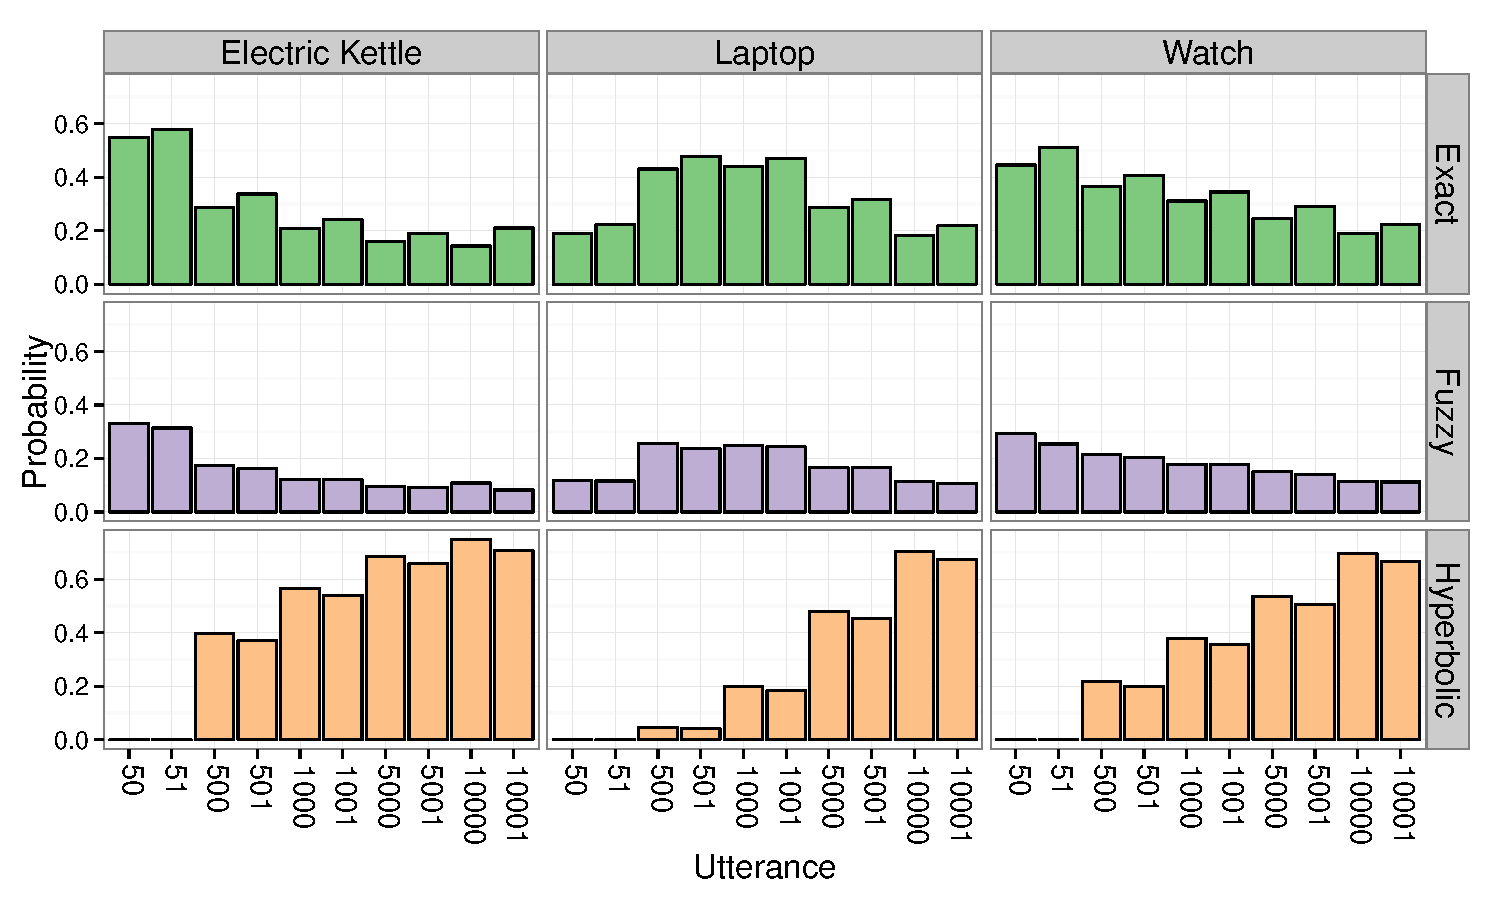
\includegraphics[width=8.7cm]{model_effects_bar_noAffect.pdf}
\caption{Hello}\label{model_effects}
\end{minipage}\hfill
\begin{minipage}[b]{.49\textwidth}
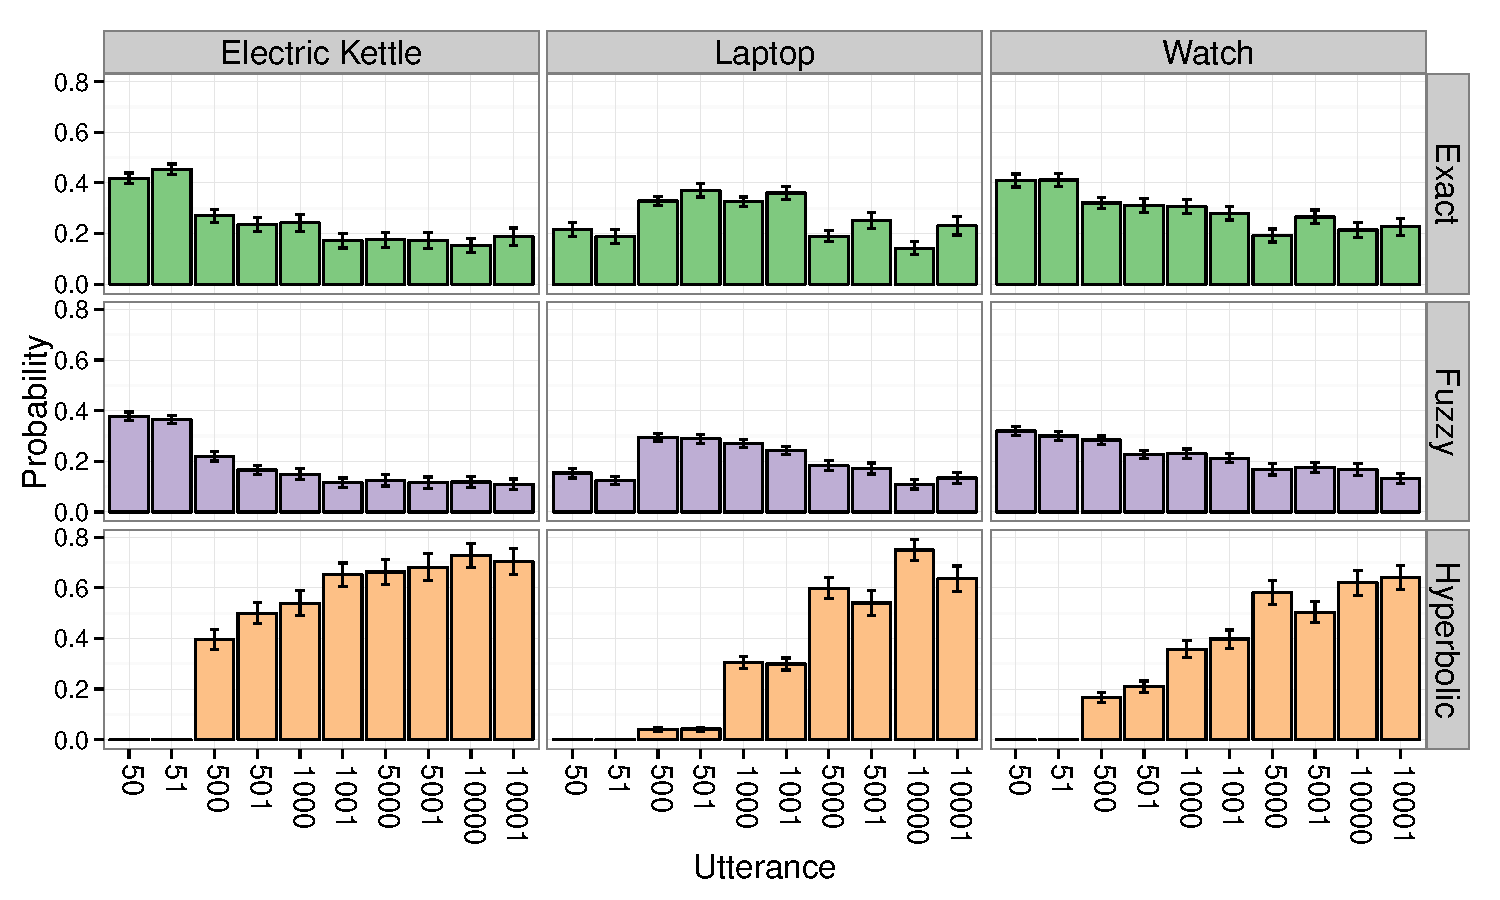
\includegraphics[width=8.7cm]{human_effects_bar_noAffect.pdf}
\caption{Vertical panels show results for the three item kinds. Horizontal panels show the three kinds of interpretations, \emph{exact}, \emph{fuzzy}, and \emph{hyperbolic}. The $x$ axis in each panel represents the utterance. The $y$ axis shows the probability of a kind of interpretation given the utterance.}\label{human_effects}
\end{minipage}
\end{figure*}


\begin{figure*}
\centering
\begin{minipage}[b]{.49\textwidth}
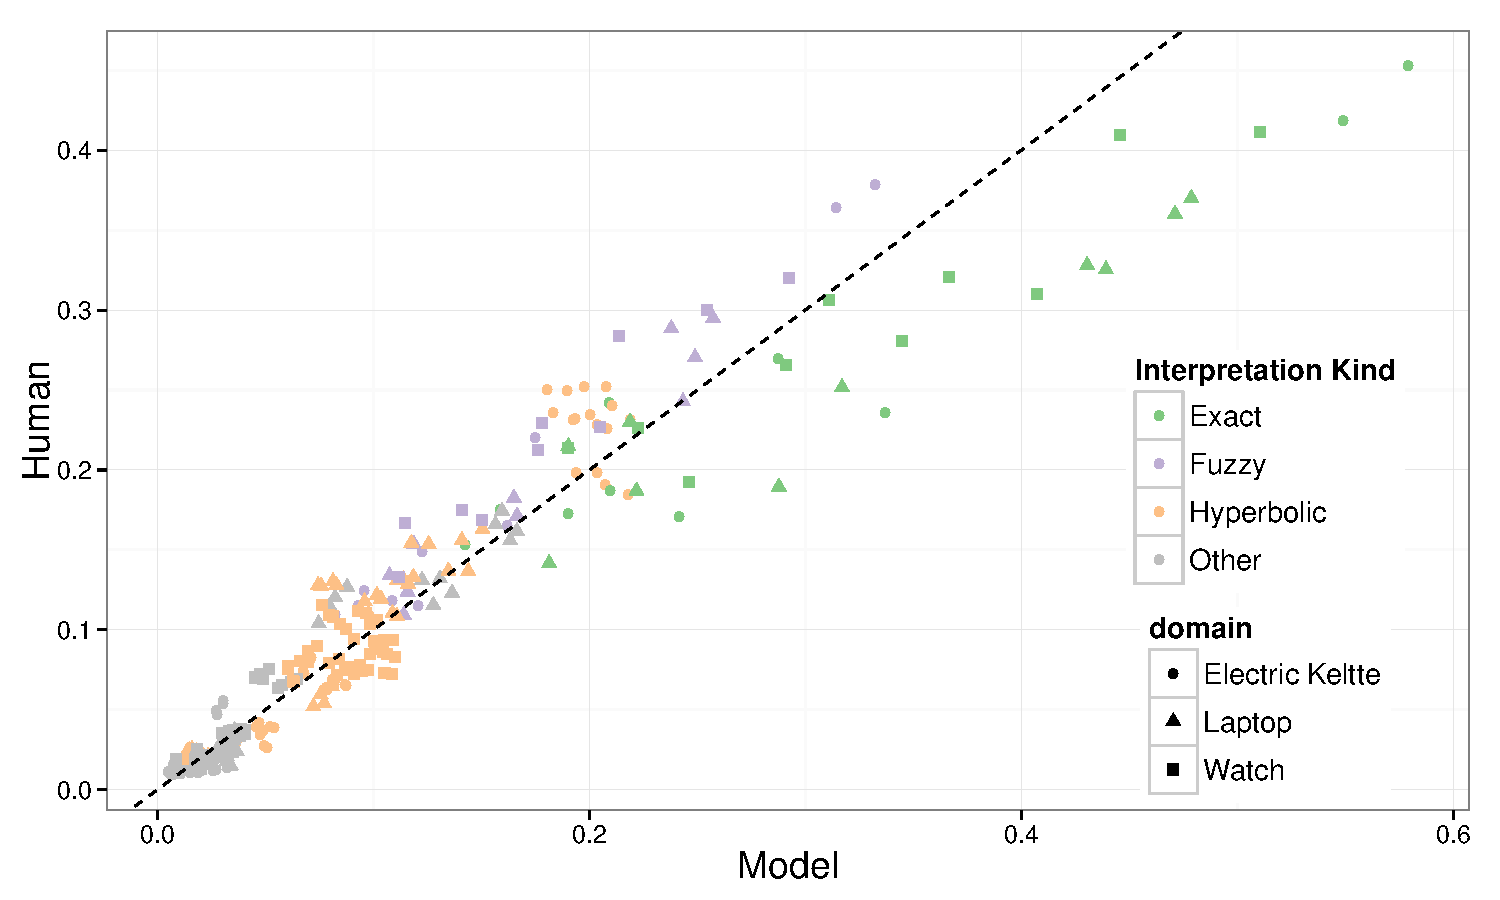
\includegraphics[width=8.7cm]{human_model_scatter.pdf}
\caption{Hello}\label{model_fit}
\end{minipage}\hfill
\begin{minipage}[b]{.4\textwidth}
\begin{tabular}{l l}
\hline
\textbf{Model} & \textbf{$R^2$}\\
\hline
Full & $0.92$\\
Uniform prior & bad \\
Uniform cost & bad \\
Uniform affect & bad \\
\hline
\end{tabular}
\label{model_fit}
\end{minipage}
\caption{We show the model and human interpretation probabilities for all $300$ items ($10$ utterances crossed with $10$ price states and $3$ item kinds. The model significantly predicts human interpretations with very high correlation ($r=0.96$, $p<0.0001$.)}
\end{figure*}

We test our model's interpretation of number expressions regarding the prices of three kinds of everyday items: \emph{electric kettles}, \emph{watches}, and \emph{laptops}. We chose to focus on price because it is a common and natural topic of conversation in which people use number expressions frequently.
% and people have good prior knowledge of the price distributions for the three kinds of items. 
%Furthermore, the price distributions are quite different from each other (e.g. $1000$ dollars is a probable price for a laptop but improbable for an electric kettle).
% QUESTION: Should we include a plot of scraped priors for these items to show that they're different?
We chose ten numbers as the set of possible price states for the three kinds of items: $S=\{50, 50', 500, 500', 1000, 1000', 5000, 5000', 10000, 10000'\}$. The ten numbers can be seen as five pairs of numbers in which each pair consists of a ``round" number state $s$ (which is a number divisable by $10$) and its ``sharp" counterpart $s'$ (which we define as $s \pm k $, $k \in \{1, 2, 3\}$).
 We assume that the space of possible utterances $U$ is the same as the space of possible price states. For example, a speaker can say, ``That electric kettle cost $u$ dollars," for $u \in U$.
 % FIXME: Notation might be confusing.
 
\subsection{Model} 
Our model considers the following five communicative goals: whether the speaker wants to convey the price precisely, imprecisely, or not at all, crossed with whether the speaker wants to convey her opinion about the price or not, minus the vacuous goal in which the speaker wants to convey nothing. We assume a uniform prior over goals. The model considers the possible price state meanings $S$ and the prior probability $P(s)$ of each price state for a given kind of item (see Experiment 2(a) in materials). It also considers the prior conditional probability $E(s)$ of a given price state being considered expensive (see Experiment 2(b) in materials). Finally, it considers the cost of each utterance $C(u)$ and assumes that sharp numbers are costlier to utter than round numbers. 

Given the formal setup of our model described in the methods section, we obtained posterior meaning distributions for each of the ten numerical utterances for each of the three item kinds. Figure \ref{full_bar} in the Appendix shows the full meaning distribution for each utterance. We broke down the interpretations into three separate kinds: \emph{exact interpretations}, which are interpretations that are identical to the utterance (e.g. when``1000" is interpreted as meaning $1000$); \emph{fuzzy interpretations}, which are interpretations that are counterpart to the utterance (e.g. ``1000" interpreted as meaning $1001$); and \emph{hyperbolic interpretations}, which are interpretations that are smaller than the utterance besides fuzzy interpretations (e.g. ``1000" interpreted as meaning $50$). The model also returns the probability of an utterance being interpreted as conveying \emph{affect} about the price being too expensive. Figure \ref{model_effects} summarizes these effects. We first see a basic effect of the prior, in which utterances that are more likely given the price prior of the item are more likely to be interpreted exactly or fuzzily (e.g. ``1000" is more likely to be interpreted exactly or fuzzily for laptops than for electric kettles). The model demonstrates the pragmatic halo effect, in which round utterances such as ``500" and ``1000" are interpreted less exactly and more fuzzily than their sharp counterparts ``501" and ``1001." It also demonstrates the hyperbole effect, in which utterances that are less likely given the price prior are more likely to be interpreted hyperbolically (e.g. ``1000" is more likely to be interpreted as $50, 51, 500,$ or $501$ for electric kettles than for laptops). We also see an interaction between halo and hyperbole, where round utterances such as ``5000" and ``10000" are more likely to be interpreted hyperbolically than their sharp counterparts.

\subsection{Experiment}
We conducted an experiment on humans' interpretation of number words using the same set of items, price states $S$, and utterances $U$ as provided to the model. Subjects read scenarios in which a buyer makes an utterance $u$ about the price of an item he just bought. Subjects rate the likelihood of the buyer thinking that the item was expensive, as well as the likelihood that the item had actually cost $s$ dollars for $s \in S$ (see Experiment 1 in materials). Figure \ref{full_bar} in the Appendix shows the full meaning distribution for each utterance. We broke down the interpretations into \emph{exact}, \emph{fuzzy}, and \emph{hyperbolic}. Figure \ref{human_effects} summarizes these effects. We see that round utterances tend to be interpreted less exactly and more fuzzily than their sharp counterparts, and utterances that are less likely given the price prior are more likely to be interpreted hyperbolically. We also see that round utterances are more likely to be interpreted hyperbolically.
%%TODO
% Figure out what stats to report here.

\subsection{Comparison}
Our model results correlate significantly with human interpretations of number words ($r=0.96$, $p<0.0001$) (Figure \ref{model_fit}). We lesion stuff and fit gets much worse.

%------------------------------------------------

\section{Discussion}

%Despite having highly standard literal meanings, numbers are often used non-literally in everyday language. 
Our behavioral results show that people often interpret numerical expressions in imprecise or non-literal ways, even in the absence of phonological cues. However, there are complex patterns in this non-literal usage: hyperbole depends on prior probability, conveys affective subtext, and interacts with the halo of round numbers.
Building upon recent theoretical work, our computational model shows that rational recursive reasoning between speaker and listener can capture these effects of pragmatic halo and hyperbole. Our model introduces an ``affect" dimension to language interpretation, such that hyperbolic utterances efficiently convey information regarding the speaker's opinion and affective state. However, the subtext conveyed by language often goes beyond the simple binary state used here. Future work will explore both the rich structure of subtext and the extension of this modeling framework to other cases of non-literal speech: ``Bayesian models can explain \emph{everything}."


%----------------------------------------------------------------------------------------
%	MATERIALS AND METHODS
%----------------------------------------------------------------------------------------

%% Optional Materials and Methods Section
%% The Materials and Methods section header will be added automatically.

\begin{materials}
\section{Model}
Here we describe our model in detail. A literal listener $L_0$ provides the base case for recursive social reasoning between the speaker and listener. $L_0$ interprets an utterance literally without taking into account the speaker's communicative goals. 

The literal listener $L_0$'s interpretation of an utterance $u$ can be given as follows:

\begin{equation}\label{eq:literallistener}
L_0(m|u) \propto \sum_{<i \in\{s, s', 0\}, j\in\{a, 0\}>}P(m | g_{<i, j>}, u).
\end{equation}

$L_0$ interprets an utterance ``$n$" with some uncertainty about the speaker's communicative goal regarding the price state $S$ and the affective subtext $A$. We represent this goal as $g_{<S, A>}$, where $g_{<s', a>}$ represent the goal to communicate both the precise price state and affective subtext, $g_{<s, 0>}$ represent the goal to communicate the imprecise price state and no affective subtext, and $g_{<0, a>}$ to communicate the affective subtext only, and so on.

$L_0$'s interpretation $m$ of an utterance ``$n$" has two parts: the price state and the affect. We represent this interpretation as $m_{<S, A>}$.
Given $g_{<s', \{a, 0\}>}$ $L_0$ interprets ``$n$" as meaning $n$ with probability $1$ given $g_{<s', \{a, 0\}>}$, as meaning $n-1$, $n$, or $n+1$ with uniform probability given $g_{<s, \{a, 0\}>}$, and as meaning the price is expensive with probability $E(n)$ when $g_{<\{s', s\}, e>}$.

The speaker $S_n$ is assumed to be a rational planner who optimizes the probability that her intended meaning $m$ will be understood by the listener $L_n$ and thus satisfy her communicative goal while minimizing the cost of the utterance. The speaker $S_n$ chooses utterances according to a softmax decision rule that describes an approximately rational planner \cite{sutton1998reinforcement}:
\begin{equation}\label{eq:speakerprob}
S_n(u | m, g) \propto e^{\lambda U_n(u | m, g)},
\end{equation}
where the constant $\lambda$ captures the degree of optimality of the speaker. (We used $\lambda=2$ in the model simulations for this section).
The speaker wants to minimize both the cost $c(u)$ of the utterance and the surprisal of the intended meaning $m$, so the utility function $U_n$ is defined by:
\begin{equation}\label{eq:speakerutility}
U_n(u | m, g) = \log (L_{n}(m | u, g)) - c(u),
\end{equation}
which combined with equation \ref{eq:speakerprob} leads to:
\begin{equation}\label{eq:speakersimplified}
S_n(u | m, g) \propto (L_{n}(m | u, g)e^{-c(u)}) ^\lambda.
\end{equation}

The listener $L_n$ performs Bayesian inference to guess the intended meaning given the prior $P$ and his internal model of the speaker. To determine the speaker's intended meaning, the listener will marginalize over the possible goals under consideration. The listener $L_n$ performs Bayesian inference to guess the intended meaning given the prior $P$ and his internal model of the speaker$S_{n-1}$.

\begin{equation}\label{eq:listenerdict}
L_n(m|u) \propto \sum_{i }P(m)P(g_i)S_{n-1}(u | m,g_i).
\end{equation}

\section{Experiment 1a: Halo and hyperbole}
$120$ subjects were recruited from Amazon's Mechanical Turk to participate in our experiment on number word interpretation. Each subject read $15$ scenarios in which a person (e.g. Bob) buys an item (e.g. a watch) and is asked by a friend whether the item is expensive. Bob responds by saying ``It cost $u$ dollars," where $u \in \{50, 50\pm k, 500, 500\pm k, 1000, 1000 \pm k, 5000, 5000 \pm k, 10000, 10000 \pm k\}$. $k$ was randomly selected from the set $\{1, 2, 3\}$ for each trial. From now on this set of prices will be referred to as $U$. Given this utterance, subjects rated the probability of Bob thinking that the item was expensive. They then rated the probability of the item costing the following amounts of money: $50$, $50\pm k$, $500$, $500\pm k$, $1000$, $1000 \pm k$, $5000$, $5000 \pm k$, $10000$, $10000 \pm k$, where $k$ was randomly selected from the set $\{1, 2, 3\}$ for each trial. From now on this set of prices will be referred to as $S$. Ratings for each price state were on a continuous scale from ``impossible" to ``Extremely likely", represented as real values between $0$ and $1$. We normalized subjects' ratings across price points for each trial to sum up to $1$. The average normalized ratings across subjects for each item/utterance pair is shown in Figure \ref{full_bar}.

\section{Experiment 1a: Affective subtext}

\section{Experiment 2a: Price prior}
To obtain people's prior knowledge of the price distributions for electric kettles, laptops, and watches, $30$ subjects were recruited from Amazon's Mechanical Turk. Each subject rated the probability of an electric kettle, laptop, and watch costing $s$ dollars, where $s \in S$. Ratings for each price state were on a continuous scale from ``impossible" to ``Extremely likely", represented as real values between $0$ and $1$. We normalized subjects' ratings across price points for each trial to sum up to $1$. The average normalized ratings across subjects for each item were taken as the prior probability distribution of item prices. These price distributions were used in the model to determine the prior probability of each price state.

\section{Experiment 2b: Affect prior}
To obtain people's prior knowledge of the affect likelihood given a price state, $30$ subjects were recruited from Amazon's Mechanical Turk. Each subject read $15$ scenarios where someone had just bought an item that cost $s$ dollars ($s \in S$). They then rated how likely the buyer would think the item was expensive on a continuous scale ranging from ``impossible" to "absolutely certain," represented as real values between $0$ and $1$. The average ratings for each item/price state pair were taken as the prior probability of an affect given a price state. This was used in the model to determine the prior probability of an affect given each price state.

\end{materials}

%----------------------------------------------------------------------------------------
%	APPENDICES (OPTIONAL)
%----------------------------------------------------------------------------------------

\appendix
\begin{figure*}[h]
\centering
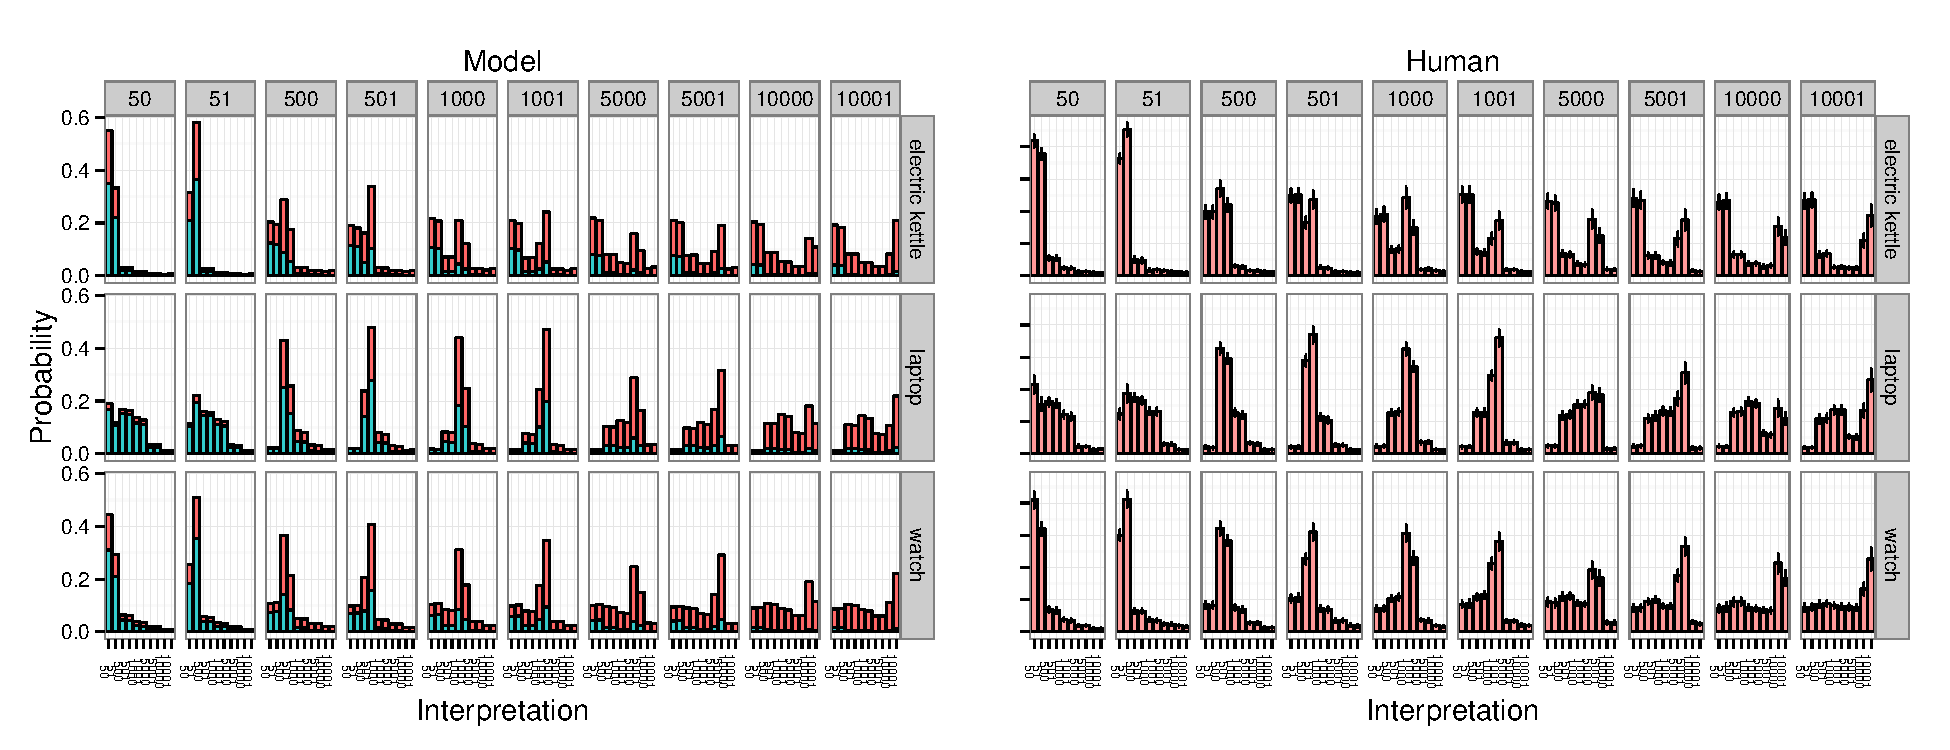
\includegraphics[width=18.6cm]{full_bar.pdf}
\caption{Hello}\label{full_bar}
\end{figure*}


\appendix[Appendix title]
An appendix with a title.

%----------------------------------------------------------------------------------------
%	ACKNOWLEDGEMENTS
%----------------------------------------------------------------------------------------

\begin{acknowledgments}
This work was partially supported by a grant from the Spanish Ministry of Science and Technology.
\end{acknowledgments}

%----------------------------------------------------------------------------------------
%	BIBLIOGRAPHY
%----------------------------------------------------------------------------------------

%% PNAS does not support submission of supporting .tex files such as BibTeX.
%% Instead all references must be included in the article .tex document. 
%% If you currently use BibTeX, your bibliography is formed because the 
%% command \verb+\bibliography{}+ brings the <filename>.bbl file into your
%% .tex document. To conform to PNAS requirements, copy the reference listings
%% from your .bbl file and add them to the article .tex file, using the
%% bibliography environment described above.  

%%  Contact pnas@nas.edu if you need assistance with your
%%  bibliography.

% Sample bibliography item in PNAS format:
%% \bibitem{in-text reference} comma-separated author names up to 5,
%% for more than 5 authors use first author last name et al. (year published)
%% article title  {\it Journal Name} volume #: start page-end page.
%% ie,
% \bibitem{Neuhaus} Neuhaus J-M, Sitcher L, Meins F, Jr, Boller T (1991) 
% A short C-terminal sequence is necessary and sufficient for the
% targeting of chitinases to the plant vacuole. 
% {\it Proc Natl Acad Sci USA} 88:10362-10366.


%% Enter the largest bibliography number in the facing curly brackets
%% following \begin{thebibliography}

\begin{thebibliography}{10}
\bibitem{BN}
M.~Belkin and P.~Niyogi, {\em Using manifold structure for partially
  labelled classification}, Advances in NIPS, 15 (2003).

\bibitem{BBG:EmbeddingRiemannianManifoldHeatKernel}
P.~B\'erard, G.~Besson, and S.~Gallot, {\em Embedding {R}iemannian
  manifolds by their heat kernel}, Geom. and Fun. Anal., 4 (1994),
  pp.~374--398.

\bibitem{CLAcha1}
R.R.~Coifman and S.~Lafon, {\em Diffusion maps}, Appl. Comp. Harm. Anal.,
  21 (2006), pp.~5--30.

\bibitem{DiffusionPNAS}
R.R.~Coifman, S.~Lafon, A.~Lee, M.~Maggioni, B.~Nadler, F.~Warner, and
  S.~Zucker, {\em Geometric diffusions as a tool for harmonic analysis and
  structure definition of data. {P}art {I}: Diffusion maps}, Proc. of Nat.
  Acad. Sci.,  (2005), pp.~7426--7431.

\bibitem{Clementi:LowDimensionaFreeEnergyLandscapesProteinFolding}
P.~Das, M.~Moll, H.~Stamati, L.~Kavraki, and C.~Clementi, {\em
  Low-dimensional, free-energy landscapes of protein-folding reactions by
  nonlinear dimensionality reduction}, P.N.A.S., 103 (2006), pp.~9885--9890.

\bibitem{DoGri}
D.~Donoho and C.~Grimes, {\em Hessian eigenmaps: new locally linear
  embedding techniques for high-dimensional data}, Proceedings of the National
  Academy of Sciences, 100 (2003), pp.~5591--5596.

\bibitem{DoGri:WhenDoesIsoMap}
D.~L. Donoho and C.~Grimes, {\em When does isomap recover natural
  parameterization of families of articulated images?}, Tech. Report Tech. Rep.
  2002-27, Department of Statistics, Stanford University, August 2002.

\bibitem{GruterWidman:GreenFunction}
M.~Gr\"uter and K.-O. Widman, {\em The {G}reen function for uniformly
  elliptic equations}, Man. Math., 37 (1982), pp.~303--342.

\bibitem{Simon:NeumannEssentialSpectrum}
R.~Hempel, L.~Seco, and B.~Simon, {\em The essential spectrum of neumann
  laplacians on some bounded singular domains}, 1991.

\bibitem{1}
Kadison, R.\ V.\ and Singer, I.\ M.\ (1959)
Extensions of pure states, {\it Amer.\ J.\ Math.\ \bf
81}, 383-400.

\bibitem{2}
Anderson, J.\ (1981) A conjecture concerning the pure states of
$B(H)$ and a related theorem. in {\it Topics in Modern Operator
Theory}, Birkha\"user, pp.\ 27-43.

\bibitem{3}
Anderson, J.\ (1979) Extreme points in sets of
positive linear maps on $B(H)$. {\it J.\ Funct.\
Anal.\
\bf 31}, 195-217.

\bibitem{4}
Anderson, J.\ (1979) Pathology in the Calkin algebra. {\it J.\
Operator Theory \bf 2}, 159-167.

\bibitem{5}
Johnson, B.\ E.\ and Parrott, S.\ K.\ (1972) Operators commuting
with a von Neumann algebra modulo the set of compact operators.
{\it J.\ Funct.\ Anal.\ \bf 11}, 39-61.

\bibitem{6}
Akemann, C.\ and Weaver, N.\ (2004) Consistency of a
counterexample to Naimark's problem. {\it Proc.\ Nat.\ Acad.\
Sci.\ USA \bf 101}, 7522-7525.

\bibitem{TSL}
J.~Tenenbaum, V.~de~Silva, and J.~Langford, {\em A global geometric
  framework for nonlinear dimensionality reduction}, Science, 290 (2000),
  pp.~2319--2323.

\bibitem{ZhaZha}
Z.~Zhang and H.~Zha, {\em Principal manifolds and nonlinear dimension
  reduction via local tangent space alignement}, Tech. Report CSE-02-019,
  Department of computer science and engineering, Pennsylvania State
  University, 2002.
\end{thebibliography}

%@article{mccarthy2004there,
%  title={�There's millions of them�: hyperbole in everyday conversation},
%  author={McCarthy, M. and Carter, R.},
%  journal={Journal of pragmatics},
%  volume={36},
%  number={2},
%  pages={149--184},
%  year={2004},
%  publisher={Elsevier}
%}
%
%@article{gibbs2000irony,
%  title={Irony in talk among friends},
%  author={Gibbs, R.W.},
%  journal={Metaphor and symbol},
%  volume={15},
%  number={1-2},
%  pages={5--27},
%  year={2000},
%  publisher={Taylor \& Francis}
%}
%
%@article{cano2003risk,
%  title={At the Risk of Exaggerating: How Do Listeners React to Hyperbole?},
%  author={Cano Mora, L.},
%  journal={Anglogermanica online: Revista electr{\'o}nica peri{\'o}dica de filolog{\'\i}a alemana e inglesa},
%  number={2},
%  pages={2--13},
%  year={2003}
%}
%
%@article{kotthoff2003responding,
%  title={Responding to irony in different contexts: On cognition in conversation},
%  author={Kotthoff, H.},
%  journal={Journal of pragmatics},
%  volume={35},
%  number={9},
%  pages={1387--1411},
%  year={2003},
%  publisher={Elsevier}
%}
%
%@article{kreuz2000production,
%  title={The production and processing of verbal irony},
%  author={Kreuz, R.J.},
%  journal={Metaphor and Symbol},
%  volume={15},
%  number={1-2},
%  pages={99--107},
%  year={2000},
%  publisher={Taylor \& Francis}
%}
%
%@article{kreuz1995two,
%  title={Two cues for verbal irony: Hyperbole and the ironic tone of voice},
%  author={Kreuz, R.J. and Roberts, R.M.},
%  journal={Metaphor and symbol},
%  volume={10},
%  number={1},
%  pages={21--31},
%  year={1995},
%  publisher={Taylor \& Francis}
%}
%
%@article{capelli1990children,
%  title={How children understand sarcasm: The role of context and intonation},
%  author={Capelli, C.A. and Nakagawa, N. and Madden, C.M.},
%  journal={Child Development},
%  volume={61},
%  number={6},
%  pages={1824--1841},
%  year={1990},
%  publisher={Wiley Online Library}
%}
%
%@inproceedings{kreuz2007lexical,
%  title={Lexical influences on the perception of sarcasm},
%  author={Kreuz, R.J. and Caucci, G.M.},
%  booktitle={Proceedings of the Workshop on Computational Approaches to Figurative Language},
%  pages={1--4},
%  year={2007},
%  organization={Association for Computational Linguistics}
%}
%
%@inproceedings{davidov2010semi,
%  title={Semi-supervised recognition of sarcastic sentences in twitter and amazon},
%  author={Davidov, D. and Tsur, O. and Rappoport, A.},
%  booktitle={Proceedings of the Fourteenth Conference on Computational Natural Language Learning},
%  pages={107--116},
%  year={2010},
%  organization={Association for Computational Linguistics}
%}
%
%@article{reyes2011mining,
%  title={Mining subjective knowledge from customer reviews: a specific case of irony detection},
%  author={Reyes, A. and Rosso, P.},
%  journal={ACL HLT 2011},
%  pages={118},
%  year={2011},
%  publisher={Citeseer}
%}
%
%@article{van2007algorithm,
%  title={Algorithm Development in Computerized Detection of Sarcasm using Vocal Cues},
%  author={van Kruijsdijk, R.},
%  year={2007}
%}
%
%@book{moreno2007creativity,
%  title={Creativity and convention: The pragmatics of everyday figurative speech},
%  author={Moreno, R.E.V.},
%  volume={156},
%  year={2007},
%  publisher={John Benjamins Publishing Co}
%}
%
%@inproceedings{bergen2012,
%title = {That's what she (could have) said: How alternative utterances affect language use},
%author={Bergen, L. and Goodman, G.D. and Levy, R.},
%year={2012},
%booktitle={Proceedings of CogSci conference},
%}
%
%
%@inproceedings{stiller2011ad,
%  title={Ad-hoc scalar implicature in adults and children},
%  author={Stiller, A. and Goodman, N.D. and Frank, M.C.},
%  booktitle={Proceedings of the 33rd Annual Meeting of the Cognitive Science Society},
%  year={2011}
%}
%
%@article{bastiaanse2011rationality,
%  title={The rationality of round interpretation},
%  author={Bastiaanse, H.},
%  journal={Vagueness in communication},
%  pages={37--50},
%  year={2011},
%  publisher={Springer}
%}
%
%@article{krifka2007approximate,
%  title={Approximate interpretation of number words: A case for strategic communication},
%  author={Krifka, M.},
%  journal={Cognitive foundations of interpretation},
%  pages={111--126},
%  year={2007}
%}
%
%@inproceedings{sauerland2007scalar,
%  title={Scalar vs. epistemic vagueness: Evidence from approximators},
%  author={Sauerland, U. and Stateva, P.},
%  booktitle={Proceedings of SALT},
%  volume={17},
%  number={0},
%  pages={228--245},
%  year={2007}
%}
%
%@article{frankgoodmanscience,
%  title={Predicting pragmatic reasoning in language games},
%  author={Frank, M.C. and Goodman, N.D.},
%  journal={Science},
%  volume={336},
%  number={6084},
%  pages={998},
%  year={2012}
%}
%
%@article{van2004signalling,
%  title={Signalling games select Horn strategies},
%  author={{van Rooij}, R.},
%  journal={Linguistics and Philosophy},
%  volume={27},
%  number={4},
%  pages={493--527},
%  year={2004},
%  publisher={Springer}
%}
%
%@article{van2008games,
%  title={Games and Quantity implicatures},
%  author={{van Rooij}, R.},
%  journal={Journal of Economic Methodology},
%  volume={15},
%  number={3},
%  pages={261--274},
%  year={2008},
%  publisher={Taylor \& Francis}
%}
%
%@article{franke2009interpretation,
%  title={Interpretation of optimal signals},
%  author={Franke, M.},
%  journal={New perspectives on games and interaction},
%  pages={297--310},
%  year={2009},
%  publisher={Amsterdam University Press}
%}
%
%
%@book{sutton1998reinforcement,
%  title={Reinforcement learning: An introduction},
%  author={Sutton, R.S. and Barto, A.G.},
%  volume={28},
%  year={1998},
%  publisher={Cambridge Univ Press}
%}
%
%@article{grice1975,
%	Author = {Grice, H.P.},
%	Journal = {1975},
%	Pages = {41--58},
%	Title = {Logic and conversation},
%	Year = {1975}}
%
%@inproceedings{jager2009pragmatic,
%  title={Pragmatic rationalizability},
%  author={J{\"a}ger, G. and Ebert, C.},
%  booktitle={Proceedings of Sinn und Bedeutung},
%  volume={13},
%  pages={1--15},
%  year={2009}
%}
%
%@article{jager2008game,
%  title={Game theory in semantics and pragmatics},
%  author={J{\"a}ger, G.},
%  journal={manuscript, University of Bielefeld},
%  year={2008}
%}
%
%@article{cho1987signaling,
%  title={Signaling games and stable equilibria},
%  author={Cho, I.K. and Kreps, D.M.},
%  journal={The Quarterly Journal of Economics},
%  volume={102},
%  number={2},
%  year={1987},
%  publisher={Oxford University Press}
%}
%
%@article{chen2008selecting,
%  title={Selecting Cheap-Talk Equilibria},
%  author={Chen, Y. and Kartik, N. and Sobel, J.},
%  journal={Econometrica},
%  volume={76},
%  number={1},
%  pages={117--136},
%  year={2008},
%  publisher={Wiley Online Library}
%}
%
%@inproceedings{goodmanstuhlmueller,
%  title={Knowledge and implicature: Modeling language understanding as social cognition},
%  author={Goodman, N.D. and Stuhlm{\"u}ller, A.},
%  booktitle={Proceedings of CogSci conference},
%  year={2012}
%}
%
%
%@article{lasersohn1999pragmatic,
%  title={Pragmatic halos},
%  author={Lasersohn, P.},
%  journal={Language},
%  pages={522--551},
%  year={1999},
%  publisher={JSTOR}
%}
%
%@book{clark1996using,
%  title={Using language},
%  author={Clark, H.H.},
%  volume={4},
%  year={1996},
%  publisher={Cambridge University Press Cambridge}
%}

%----------------------------------------------------------------------------------------

\end{article}

%----------------------------------------------------------------------------------------
%	FIGURES AND TABLES
%----------------------------------------------------------------------------------------

%% Adding Figure and Table References
%% Be sure to add figures and tables after \end{article}
%% and before \end{document}

%% For figures, put the caption below the illustration.
%%
%% \begin{figure}
%% \caption{Almost Sharp Front}\label{afoto}
%% \end{figure}

%% For Tables, put caption above table
%%
%% Table caption should start with a capital letter, continue with lower case
%% and not have a period at the end
%% Using @{\vrule height ?? depth ?? width0pt} in the tabular preamble will
%% keep that much space between every line in the table.

%% \begin{table}
%% \caption{Repeat length of longer allele by age of onset class}
%% \begin{tabular}{@{\vrule height 10.5pt depth4pt  width0pt}lrcccc}
%% table text
%% \end{tabular}
%% \end{table}

%% For two column figures and tables, use the following:

%% \begin{figure*}
%% \caption{Almost Sharp Front}\label{afoto}
%% \end{figure*}

%% \begin{table*}
%% \caption{Repeat length of longer allele by age of onset class}
%% \begin{tabular}{ccc}
%% table text
%% \end{tabular}
%% \end{table*}

%----------------------------------------------------------------------------------------

\end{document}